\documentclass[conference]{IEEEtran}
\usepackage{cite,amsmath,graphicx,booktabs,url}
\graphicspath{{../results_final/}}
\title{Complementary Voice and Face Cues for Multimodal Deepfake Detection}
\author{\IEEEauthorblockN{Aryavart Singh Payal}\IEEEauthorblockA{CSET 346: Natural Language Processing\\Project PJ\_07}}
\begin{document}\maketitle
\begin{abstract}
Audio-video deepfakes may manipulate voice, face, or both, leaving single-stream detectors without relevant evidence. We evaluate a lightweight verifier on a 998-clip, speaker-disjoint subset of FakeAVCeleb v1.2. Frozen wav2vec 2.0 and CLIP representations feed separate logistic-regression classifiers; probabilities are averaged, and a validation-tuned abstention band produces REAL, FAKE, or UNCERTAIN. In pooled five-fold evaluation, voice-only, face-only, and fused ROC-AUC are 0.817, 0.746, and 0.900. The system answers 83.8\% of clips at 86.6\% accuracy among answered clips. Fusion improves ranking, transcripts do not improve detection, and face-swap-only clips remain difficult. Published FakeAVCeleb baselines are included as context, with protocol differences stated explicitly.
\end{abstract}
\begin{IEEEkeywords}deepfake detection, audio-visual learning, fusion, abstention, explainability\end{IEEEkeywords}
\section{Introduction}
A clip may contain a manipulated voice, face, or both. Voice-only detection is poorly suited to face swaps with genuine speech, while visual detection can miss cloned speech paired with an authentic face. We examine modality complementarity, fusion behavior, and uncertainty reporting on FakeAVCeleb. This empirical study compares modality baselines and fusion strategies, evaluates an abstaining verifier with stream-level explanations, and reports category and group error patterns. We do not propose a new encoder.
\section{Published Baseline}
Khalid \emph{et al.} introduced FakeAVCeleb and evaluated unimodal, ensemble, and multimodal detectors \cite{khalid}. Their appendix reports AUCs 0.533, 0.688, and 0.662 for Multimodal-1, Multimodal-2, and CDCN.
\begin{table}[t]\caption{Published FakeAVCeleb scores and this study}\label{tab:base}\centering\footnotesize
\begin{tabular}{lll}\toprule System&AUC&Evaluation\\\midrule
Multimodal-1 \cite{khalid}&0.533&Published\\
Multimodal-2 \cite{khalid}&0.688&Published\\
CDCN \cite{khalid}&0.662&Published\\
Ours: voice&0.817&5-fold speaker-disjoint OOF\\
Ours: face&0.746&5-fold speaker-disjoint OOF\\
Ours: fused&0.900&5-fold speaker-disjoint OOF\\\bottomrule\end{tabular}\end{table}
The table is contextual, not a controlled ranking. We use a selected 998-clip subset and speaker-disjoint folds; the baseline paper does not report this same evaluation protocol. Direct claims require rerunning those methods on identical clips and folds.
\section{Data and Methods}
FakeAVCeleb v1.2 contains celebrity clips with genuine and generated audio-video manipulations \cite{khalid}. We use all 500 real clips and randomly sample 166 clips from each fake category (RVFA, FVRA, FVFA), using seed 42. The balanced subset contains 998 clips from 500 speakers. RVRA is real video and audio; RVFA is cloned voice with real video; FVRA is face swap with real audio; FVFA contains both manipulations. Clips without usable audio or image features were excluded. Folds are speaker-disjoint. The dataset is available for non-commercial research and education under CC BY 4.0, with downloads by request; the team must confirm it accepted the access terms before publication \cite{fakeavlicense}. Media are not redistributed.
Audio is resampled to 16 kHz, limited to about ten seconds, and encoded with frozen wav2vec 2.0-base \cite{baevski}. Time-pooled hidden states are averaged over 13 layers (768 dimensions). Three sampled frames use detected face crops with center-crop fallback and frozen CLIP ViT-B/32 embeddings, averaged and renormalized (512 dimensions) \cite{radfordclip}. Whisper-base produces English transcripts \cite{radfordwhisper}; transcript features are evaluated but excluded from final scoring.
Each stream uses standardized features and class-balanced logistic regression. Regularization and thresholds are selected on speaker-disjoint validation data. The fused probability is
\begin{equation}p_f(x)=\frac{p_v(x)+p_i(x)}{2}.\end{equation}
A validation-tuned cutoff gives REAL or FAKE; a band around it, targeting about 15\% abstention on validation, gives UNCERTAIN. Explanations name the stream suspected of manipulation from its score; they are not independent causal explanations.
\section{Results}
On the main fixed split, voice, face, CLIP transcript, and TF-IDF transcript achieve AUC 0.825, 0.797, 0.620, and 0.484. Early voice-face fusion reaches 0.925; adding transcripts lowers it to 0.915. On repeated speaker-disjoint partitions, early concatenation reaches 0.937, late mean 0.922, and gated fusion with modality dropout 0.938. These method-comparison scores are distinct from the final estimate.
Pooled five-fold out-of-fold voice, face, and fused AUC are 0.817, 0.746, and 0.900. Across ten alternative speaker partitions, the Kaggle feature run gives fused AUC 0.909 plus or minus 0.013. Although numerically above the published scores in Table~\ref{tab:base}, subset and protocol differences prevent interpreting this as a direct performance win.
In a modality ablation, voice-plus-face late fusion reaches AUC 0.941, versus 0.834 voice, 0.786 face, and 0.624 transcript. Adding transcript lowers AUC to 0.927. Voice alone has 0.036 accuracy on face-swap-only cases in this split. Leave-one-manipulation-type-out AUC falls from 0.93--0.95 on seen types to 0.76--0.78 on a held-out type. This noisy within-dataset result is not cross-dataset generalization.
The final system has 83.8\% coverage and 86.6\% accuracy among answered clips; counting abstentions as incorrect gives 72.5\% over all clips. Of 162 UNCERTAIN predictions, 77 are real and 85 fake. Answered-clip accuracy is 99.2\% for cloned-voice fakes, 56.1\% for face-swap-only fakes, and 100\% for combined manipulations.
\begin{figure}[t]\centering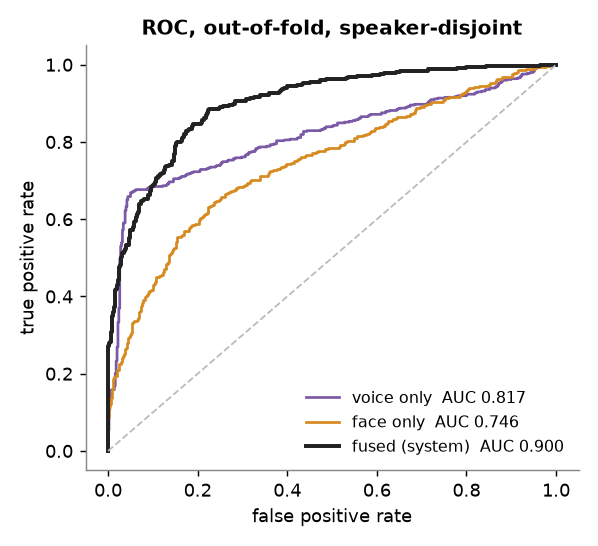
\includegraphics[width=\linewidth]{fig2_roc.png}\caption{Pooled out-of-fold ROC curves.}\label{fig:roc}\end{figure}
\begin{figure}[t]\centering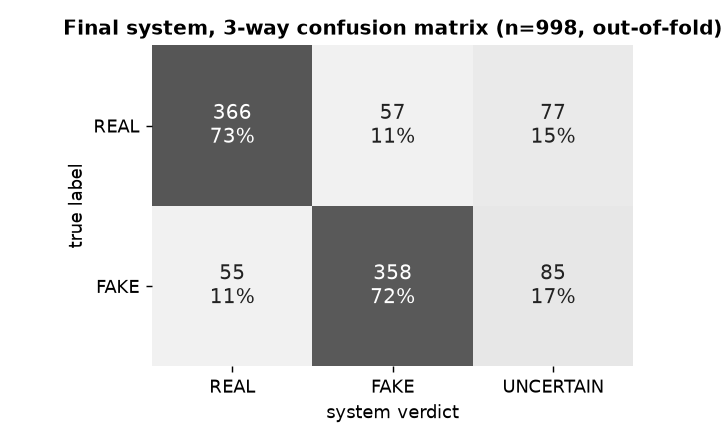
\includegraphics[width=\linewidth]{fig1_confusion_3way.png}\caption{Three-way out-of-fold confusion counts.}\label{fig:cm}\end{figure}
Explanation stream flags match audio manipulation at 97.6\% and video manipulation at 77.2\%; the exact four-way pattern is correct in 75.5\%. Among 415 FAKE verdicts, deleting the named stream cancels 42.7\%, versus 0\% when deleting the other stream. This tests dependence under one perturbation, not general causal faithfulness. Recombined genuine voice-face pairs from different speakers are called REAL in 70.6\% of cases; the system is not an identity-matching detector.
False-alarm rates range from 8.8\% to 21.2\% across ethnicity labels and 9.1\% to 17.7\% across sex labels. East Asian speakers have 0.816 answer-only accuracy and 20.9\% miss rate; American Caucasian speakers have 21.2\% false-alarm rate. These are descriptive single-dataset observations without significance tests.
\begin{figure}[t]\centering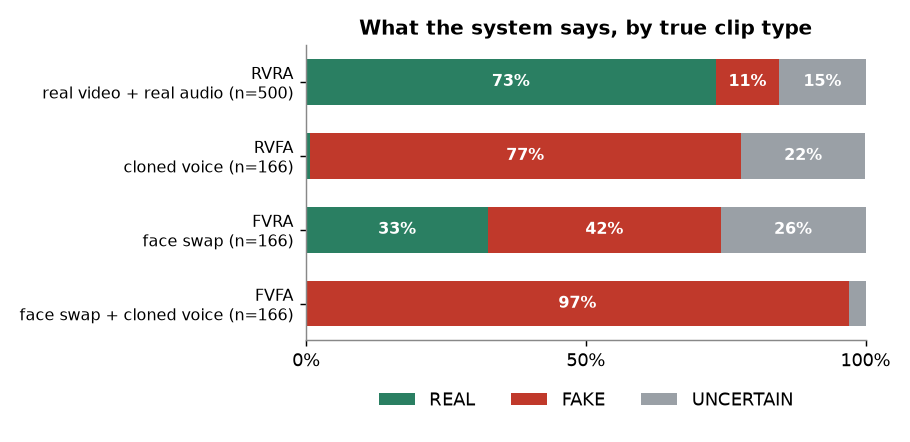
\includegraphics[width=\linewidth]{fig3_verdict_by_category.png}\caption{Verdict distribution by clip category.}\label{fig:cat}\end{figure}
\begin{figure}[t]\centering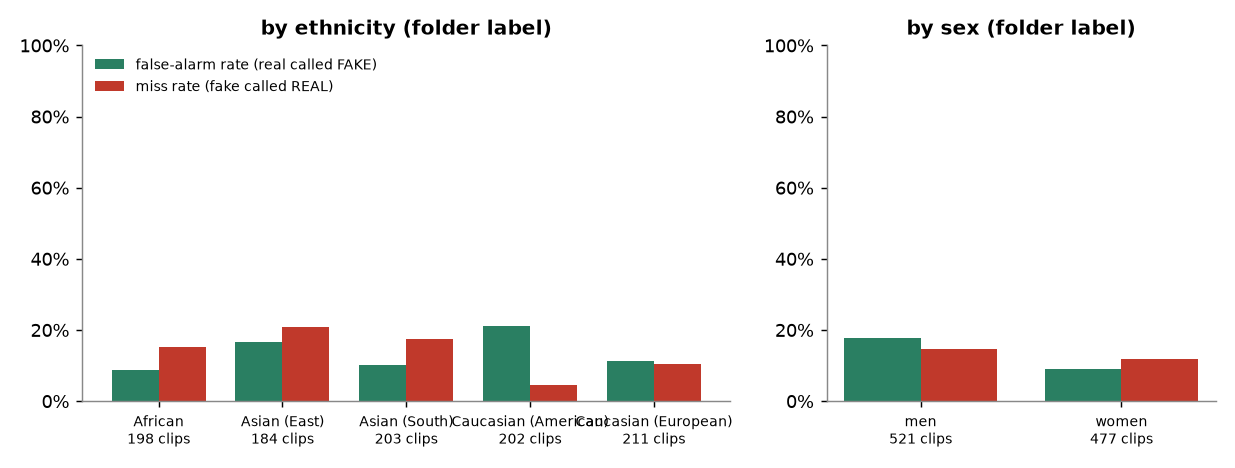
\includegraphics[width=\linewidth]{fig5_bias_audit.png}\caption{False-alarm and miss rates by folder-derived group labels.}\label{fig:bias}\end{figure}
\section{Discussion}
Voice and face streams capture different manipulation types. Simple fusion performs similarly to more complex heads in these experiments and provides a useful small-data reference. Averaging does not resolve all conflicting evidence, and face-swap-only detection remains weak. Abstention routes 16.2\% of clips for review. Transcript features do not help on this dataset and pipeline. Future work should test synchronization and identity consistency and evaluate another dataset.
\section{Limitations and Ethics}
This study uses one dataset and selected subset. Temporal pooling and three averaged frames discard fine-grained cues; CLIP is a semantic image encoder rather than a forensic detector. Cross-dataset robustness and calibrated confidence are untested. No human evaluation of explanations was run. We inspected the 15 highest-ranked scored errors in the saved out-of-fold error table: 11 are face-swap-only fakes called REAL and four are genuine clips called FAKE. Face evidence is weak or conflicts with voice scores in most false negatives; false positives often have both scores above their decision thresholds. This is a feature-level case audit, not a review of the source videos.
FakeAVCeleb contains real people's faces and voices and requires controlled research access. Verify official access and redistribution terms before publication. Folder-derived labels and observed group gaps require broader audits. A false FAKE verdict can discredit genuine media; this prototype should support human review, not serve as evidence. Do not redistribute source clips or identifying metadata.
\section{Conclusion}
On a speaker-disjoint FakeAVCeleb subset, pooled fusion improves AUC over voice and face alone (0.900 versus 0.817 and 0.746). The verifier answers 83.8\% of clips at 86.6\% answer-only accuracy, with persistent weakness on face-swap-only clips. Earlier FakeAVCeleb scores are contextual because protocols differ. Cross-dataset evaluation, forensic visual features, and human explanation evaluation remain needed.
\begin{thebibliography}{5}
\bibitem{khalid} H. Khalid, S. Tariq, M. Kim, and S. S. Woo, \textquotedblleft FakeAVCeleb: A Novel Audio-Video Multimodal Deepfake Dataset,\textquotedblright\ arXiv:2108.05080v4, 2022. [Online]. Available: \url{https://arxiv.org/abs/2108.05080}
\bibitem{baevski} A. Baevski, Y. Zhou, A. Mohamed, and M. Auli, \textquotedblleft wav2vec 2.0: A Framework for Self-Supervised Learning of Speech Representations,\textquotedblright in \emph{Advances in Neural Information Processing Systems}, vol. 33, 2020.
\bibitem{radfordclip} A. Radford \emph{et al.}, \textquotedblleft Learning Transferable Visual Models From Natural Language Supervision,\textquotedblright in \emph{Proc. Int. Conf. Mach. Learn.}, 2021, pp. 8748--8763.
\bibitem{radfordwhisper} A. Radford \emph{et al.}, \textquotedblleft Robust Speech Recognition via Large-Scale Weak Supervision,\textquotedblright in \emph{Proc. Int. Conf. Mach. Learn.}, vol. 202, 2023, pp. 28492--28518.
\bibitem{fakeavlicense} DASH Lab, \textquotedblleft FakeAVCeleb License,\textquotedblright accessed Nov. 25, 2026. [Online]. Available: \url{https://sites.google.com/view/fakeavcelebdash-lab/license}
\end{thebibliography}
\end{document}
